\documentclass{article}

\usepackage{fancyhdr}
\usepackage{extramarks}
\usepackage{amsmath}
\usepackage{amsthm}
\usepackage{amsfonts}
\usepackage{tikz}
\usepackage[plain]{algorithm}
\usepackage{algpseudocode}
\usepackage[shortlabels]{enumitem}
\usepackage{mathtools}
\usepackage{amssymb}
\usepackage{hyperref}
\usepackage{tikz}
\usepackage{pgfplots}

\usetikzlibrary{automata,positioning}

%
% Basic Document Settings
%

\topmargin=-0.45in
\evensidemargin=0in
\oddsidemargin=0in
\textwidth=6.5in
\textheight=9.0in
\headsep=0.25in

\linespread{1.1}

\pagestyle{fancy}
\lhead{\hmwkAuthorName}
\chead{\hmwkClassTime (\hmwkClassInstructor): \hmwkTitle}
\lfoot{\lastxmark}
\cfoot{\thepage}

\renewcommand\headrulewidth{0.4pt}
\renewcommand\footrulewidth{0.4pt}

\setlength\parindent{0pt}

%
% Create Problem Sections
%

\newcommand{\enterProblemHeader}[1]{
    \nobreak\extramarks{}{Problem \arabic{#1} continued on next page\ldots}\nobreak{}
    \nobreak\extramarks{Problem \arabic{#1} (continued)}{Problem \arabic{#1} continued on next page\ldots}\nobreak{}
}

\newcommand{\exitProblemHeader}[1]{
    \nobreak\extramarks{Problem \arabic{#1} (continued)}{Problem \arabic{#1} continued on next page\ldots}\nobreak{}
    \stepcounter{#1}
    \nobreak\extramarks{Problem \arabic{#1}}{}\nobreak{}
}

\setcounter{secnumdepth}{0}
\newcounter{partCounter}
\newcounter{homeworkProblemCounter}
\setcounter{homeworkProblemCounter}{1}
\nobreak\extramarks{Problem \arabic{homeworkProblemCounter}}{}\nobreak{}

\newcommand{\hmwkTitle}{Problem Set 5}
\newcommand{\hmwkDueDate}{April 30, 2024}
\newcommand{\hmwkClass}{Introduction to Economics}
\newcommand{\hmwkClassTime}{ECON 101}
\newcommand{\hmwkClassInstructor}{Robert McDonough}
\newcommand{\hmwkAuthorName}{\textbf{Rushil Umaretiya}}

%
% Title Page
%

\title{
    \vspace{2in}
    \textmd{\textbf{\hmwkClass:\ \hmwkTitle}}\\
    \normalsize\vspace{0.1in}\small{\textbf{Due\ on\ \hmwkDueDate\ at 11:59pm}}\\
    \normalsize\text{Tuesday/Thursday 3:30-4:45, Genome Sciences 100}\\
    \vspace{0.1in}\large{\textit{\hmwkClassInstructor\ - \hmwkClassTime}}
    \vspace{3in}
}

\author{\hmwkAuthorName\\\small{rumareti@unc.edu}}
\date{}

\renewcommand{\part}[1]{\textbf{\large Part \Alph{partCounter}}\stepcounter{partCounter}\\}

%
% Various Helper Commands
%

% Useful for algorithms
\newcommand{\alg}[1]{\textsc{\bfseries \footnotesize #1}}

% For derivatives
\newcommand{\deriv}[1]{\frac{\mathrm{d}}{\mathrm{d}x} (#1)}

% For partial derivatives
\newcommand{\pderiv}[2]{\frac{\partial}{\partial #1} (#2)}

% Integral dx
\newcommand{\dx}{\mathrm{d}x}

% Alias for the Solution section header
\newcommand{\solution}{\textbf{\large Solution}}

\newcommand{\question}[1]{\pagebreak\section{Question #1}}

% Probability commands: Expectation, Variance, Covariance, Bias
\newcommand{\E}{\mathrm{E}}
\newcommand{\Var}{\mathrm{Var}}
\newcommand{\Cov}{\mathrm{Cov}}
\newcommand{\Bias}{\mathrm{Bias}}

\begin{document}

\maketitle

\question{1}

For this question, you will consider McDonough's Eugene Oregon's most popular fast-food restaurant, owned by Robert. The table below includes information about McDonough's costs in the short run.

\begin{enumerate}[(a)]
    \item Fill in the table below with all of the missing values, rounding to the nearest cent.
    
    \begin{table}[h]
        \centering
        \begin{tabular}{l|l|l|l|l|l|l|l}
        
        \textbf{Quantity of Hamburgers} & TFC & TVC & TC & AFC & AVC & ATC & MC \\ \hline \hline
        0 & \textbf{\$100} & \textbf{\$0} & \$100 & - & - & - & - \\ \hline
        1,000 & \$100 & \textbf{\$800} & \$900 & \$0.10 & \$0.80 & \$0.90 & \$0.80 \\ \hline
        2,000 & \$100 & \$1,000 & \$1,100 & \$0.05 & \textbf{\$0.50} & \$0.55 & \$0.20 \\ \hline
        3,000 & \$100 & \textbf{\$1,400} & \$1,500 & \$0.033 & \$0.47 & \$0.50 & \$0.40 \\ \hline
        4,000 & \$100 & \$2,100 & \$2,200 & \$0.025 & \$0.525 & \textbf{\$0.55} & \$0.70 \\ \hline
        5,000 & \$100 & \$3,000 & \$3,100 & \$0.02 & \$0.60 & \$0.62 & \textbf{\$0.90} \\ \hline
        \end{tabular}
    \end{table}

    \item Recall that we discussed how average variable cost can be a useful signal for where diminishing marginal returns (DMR) starts to occur. Based on that observation, how many hamburgers is McDonough's producing when DMR starts?
    
    As production increases from 0 to 3,000 hamburgers, average variable cost is falling. However, as production increases from 3,000 to 4,000 hamburgers, average variable cost is rising. This increase from \$0.47 to \$0.525 in the AVC between 3,000 and 4,000 hamburgers indicates that McDonough's starts experiencing diminishing marginal returns after producing 3,000 hamburgers.

    \item Why does average fixed cost keep falling as McDonough's makes more hamburgers? Explain briefly why this fact is useful to a business.
    
    Average fixed cost keeps falling as McDonough's makes more hamburgers because fixed costs are spread over a larger number of hamburgers. This is useful to a business because it means that the business is becoming more efficient as it produces more hamburgers, which can help the business increase its profit margins.

    \item Assume that McDonough's operates in a competitive market, so that the firm is a price taker. If the price of a hamburger is \$0.70, how many hamburgers should McDonough's produce and sell?
    
    To maximize profit, McDonough's should produce and sell hamburgers until marginal cost equals marginal revenue. At a price of \$0.70, McDonough's should produce and sell 4,000 hamburgers.

    \item Assume that the fixed and variable costs shown above include opportunity costs. If the price of a hamburger is \$0.70, you should find that McDonough's is making an economic profit. How much total profit is McDonough making, and how large is the profit margin on each hamburger?
    
    At a price of \$0.70, McDonough's total cost is \$2,200, and total revenue is \$2,800. This means that McDonough's is making an economic profit of \$600. The profit margin on each hamburger is \$0.15.

    \pagebreak

    \item Eugene has many other hamburger restaurants. Graph McDonough's MC and ATC curves, as well as McDonough's MR curve. Alongside this, graph the market supply and demand for hamburgers in Eugene, and visualize how this market leads to the output level you found in (d).
    
    \begin{center}
        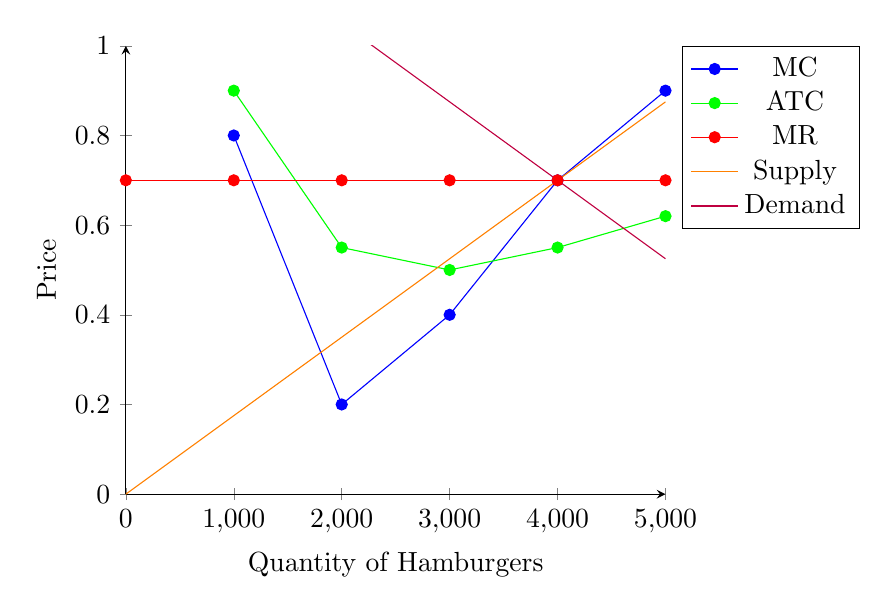
\begin{tikzpicture}
            \begin{axis}[
                axis lines = left,
                xlabel = Quantity of Hamburgers,
                ylabel = Price,
                ymin=0, ymax=1,
                xmin=0, xmax=5000,
                legend pos=outer north east,
            ]

            \addplot[
                color=blue,
                mark=*,
            ]
            coordinates {
                (1000, 0.80)
                (2000, 0.20)
                (3000, 0.40)
                (4000, 0.70)
                (5000, 0.90)
            };
            \addlegendentry{MC}

            \addplot[
                color=green,
                mark=*,
            ]
            coordinates {
                (1000, 0.90)
                (2000, 0.55)
                (3000, 0.50)
                (4000, 0.55)
                (5000, 0.62)
            };
            \addlegendentry{ATC}

            % create a plot with given points from the table for McDonough's MR

            \addplot[
                color=red,
                mark=*,
            ]
            coordinates {
                (0, 0.70)
                (1000, 0.70)
                (2000, 0.70)
                (3000, 0.70)
                (4000, 0.70)
                (5000, 0.70)
            };
            \addlegendentry{MR}


            \addplot[
                color=orange,
                domain=0:5000,
            ]{(.7*x)/4000};
            \addlegendentry{Supply}

            \addplot[
                color=purple,
                domain=0:5000,
            ]{1.4 - (.7*x)/4000};
            \addlegendentry{Demand}

            \end{axis}
        \end{tikzpicture}
    \end{center}

    \item In the long run, it is easy to enter or exit the fast-food industry in Eugene. How would you expect McDonough's economic profits to change in the long run. Explain your answer briefly.

    In the long run, McDonough's economic profits will decrease. As McDonough's economic profits increase, other firms will enter the market, increasing the supply of hamburgers and decreasing the price of hamburgers. This will decrease McDonough's economic profits until they reach zero.

\end{enumerate}

\pagebreak

\question{2}

Here you will consider Martin Byrde, who owns Byrde's Laundromat. Byrde's is the only laundromat in the Lake of the Ozarks, a popular midwestern vacation spot, making Mr. Byrde a monopolist. During the summer tourist season, the hourly demand for using one of Byrde's washing machines is given by the equation:

\begin{align*}
    P &= \$29 - \$0.20Q_D
\end{align*}

and Byrde's marginal revenue curve is given by the equation:

\begin{align*}
    MR &= \$29 - \$0.40Q_D
\end{align*}

In the short run, the marginal cost to Martin to use one of his washing machines is constant, at MC = \$1.

\begin{enumerate}[(a)]
    \item What price will Byrde set to use one of his washing machines, and how much hourly demand will there be at that price?
    
    To find the price Byrde will set to use one of his washing machines, we set marginal revenue equal to marginal cost:

    \begin{align*}
        MR &= MC \\
        \$29 - \$0.40Q_D &= \$1 \\
        Q_D &= 70 \\
        P &= \$29 - \$0.20(70) \\
        P &= \$15
    \end{align*}

    Byrde will set the price to use one of his washing machines at \$15, and there will be 70 machines demanded hourly at that price.

    \item Graph out (roughly/approximately) the demand curve, marginal revenue curve, marginal cost curve, and average total cost curve for Byrde's business.
    
    \begin{center}
        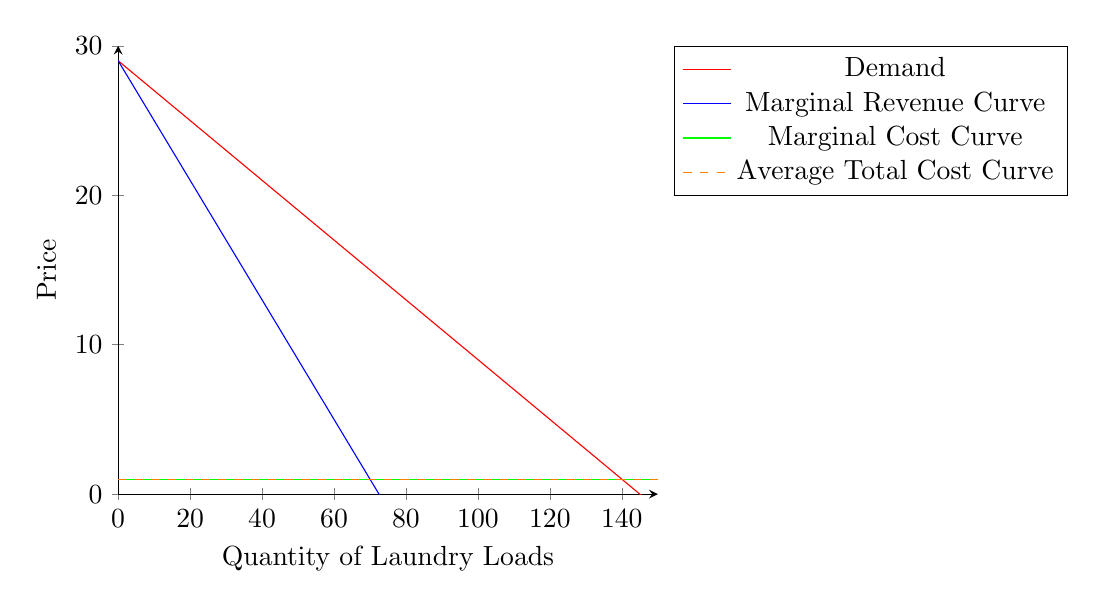
\begin{tikzpicture}
            \begin{axis}[
                axis lines = left,
                xlabel = Quantity of Laundry Loads,
                ylabel = Price,
                ymin=0, ymax=30,
                xmin=0, xmax=150,
                legend pos=outer north east,
            ]
            %Below the red parabola is defined
            \addplot [
                domain=0:150, 
                samples=100, 
                color=red,
            ]
            {29 - 0.20*x};
            \addlegendentry{Demand}

            \addplot [
                domain=0:150, 
                samples=100, 
                color=blue,
            ]
            {29 - 0.40*x};
            \addlegendentry{Marginal Revenue Curve}

            \addplot [
                domain=0:150, 
                samples=100, 
                color=green
            ]
            {1};
            \addlegendentry{Marginal Cost Curve}

            \addplot [
                domain=0:150, 
                samples=100, 
                color=orange,
                dashed
            ]
            {1};
            \addlegendentry{Average Total Cost Curve}
            \end{axis}
        \end{tikzpicture}
    \end{center}

    \item Calculate producer surplus, consumer surplus, and deadweight loss in the laundromat market in Lake of the Ozarks.
    
    For producer and consumer surplus, we can use the following formulas:
    \begin{align*}
        PS &= \frac{1}2 \times \text{Quantity} \times (\text{Price} - \text{Marginal Cost}) \\
        PS &= \frac{1}{2} \times 70 \times (15 - 1) \\
        PS &= 490 \\
        CS &= \frac{1}2 \times \text{Quantity} \times (\text{Maximum Willing to Pay} - \text{Price}) \\
        CS &= \frac{1}{2} \times 70 \times (29 - 15) \\
        CS &= 490 \\
    \end{align*}
    For DWL, we first need to find competitve quantity (where MC = P):
    \begin{align*}
        MC = P \\
        \$29 - \$0.20Q_c &= \$1 \\
        Q_c &= 140 \\
        DWL &= \frac{1}{2} \times (Q_c - Q) \times (\text{Price} - \text{Marginal Cost}) \\
        DWL &= \frac{1}{2} \times (140 - 70) \times (15 - 1) \\
        DWL &= 490
    \end{align*}

    It seems that we've found that producer surplus, consumer surplus, and deadweight loss are all equal to \$490.

\end{enumerate}

As discussed in class, monopolists under-produce because they see the
marginal revenue of extra output as being lower than the price they
receive for selling that extra output, and this is because of the output
and discount effects. We can actually see these two effects with some
simple math.


\begin{enumerate}[(a)]
    \setcounter{enumi}{3}
    \item Using the price function, calculate the price Byrde's will charge if it sells 70 laundry loads per hour, or 71 loads per hour.
    
    To find the price Byrde's will charge if it sells 71 laundry loads per hour, we plug 71 into the price function:
    \begin{align*}
        P &= \$29 - \$0.20(71) \\
        P &= \$14.80
    \end{align*}
    \pagebreak
    \item Using the prices you just found, calculate the total revenue Byrde's will get from selling 70 versus 71 loads of laundry, and use this to calculate marginal revenue (note: this will give you a slightly different number for MR than plugging 71 into the marginal revenue function. That is okay. On an exam, I would be very clear about how I ask you to calculate marginal revenue. If you are curious about why they are different, you can ask me or one of the TAs, but you are not expected to know why.)
    
    \begin{align*}
        MR &= (71 \times \$14.80) - (70 \times \$15) \\
        MR &= \$1050.8 - \$1050 \\
        MR &= \$0.80
    \end{align*}
    
    \item If Byrde's chooses to sell 71 laundry loads per hour, they must give a discount to all 70 of the previous customers to do so. How large would this discount be per customer? If you add this discount up for 70 people, how much money will Byrde's lose out on when it lowers prices?
    
    The discount per customer would be the difference between the price Byrde's would charge if it sold 70 laundry loads per hour and the price it would charge if it sold 71 laundry loads per hour:

    \begin{align*}
        \text{Discount per Customer} &= \$15 - \$14.80 \\
        \text{Discount per Customer} &= \$0.20 \\
        \text{Total Discount} &= 70 \times \$0.20 \\
        \text{Total Discount} &= \$14
    \end{align*}

    \item Given everything you've done so far, what is the value of the discount effect from selling 71 loads of laundry, and what is the value of the output effect?
    
    The value of the discount effect is \$14, and the value of the output effect is \$0.80.

\end{enumerate}
\end{document}